\subsection*{\sffamily \large The implicit solvent model}

The implicit solvent model\cite{RouxSimonson1999,DecherchiETal2015} can be described mathematically as a coupled system of partial differential equations, where the Poisson-Boltzmann governs in the solvent region ($\Omega_1$ in Figure \ref{fig:implicit_molecule}), and the Poisson equation in the solute region ($\Omega_2$ in Figure \ref{fig:implicit_molecule}). These regions are interfaced by the molecular surface ($\Gamma$), where the potential ($\phi$) and electric displacement ($\epsilon\partial\phi/\partial\mathbf{n}$) are continuous. 
%
\begin{align}\label{eq:pbe}
\nabla^2\phi_1(\mathbf{x}) &= \tfrac{1}{\epsilon_1}\sum_{k=1}^{N_q} q_k\delta(\mathbf{x},\mathbf{x}_k) \quad  \mathbf{x} \in \Omega_1\nonumber\\
\left(\nabla^2 - \kappa^2\right)\phi_2(\mathbf{x})  &= 0 \quad\mathbf{x}\in\Omega_2\nonumber\\
\phi_1(\mathbf{x})  = \phi_2 (\mathbf{x}), &\quad \epsilon_1\frac{\partial\phi_1}{\partial\mathbf{n}}(\mathbf{x})  = \epsilon_2\frac{\partial\phi_2}{\partial\mathbf{n}}(\mathbf{x})  \quad \mathbf{x}\in \Gamma. 
\end{align}
%
Here, $\epsilon_1$ and $\epsilon_2$ are the dielectric constants in the solute and solvent, respectively, $\kappa$ is the inverse of the Debye length, related with the salt concentration, and $q_k$ are the values of the partial charges, located at $\mathbf{x}_k$.

\begin{figure}[h]
\centering
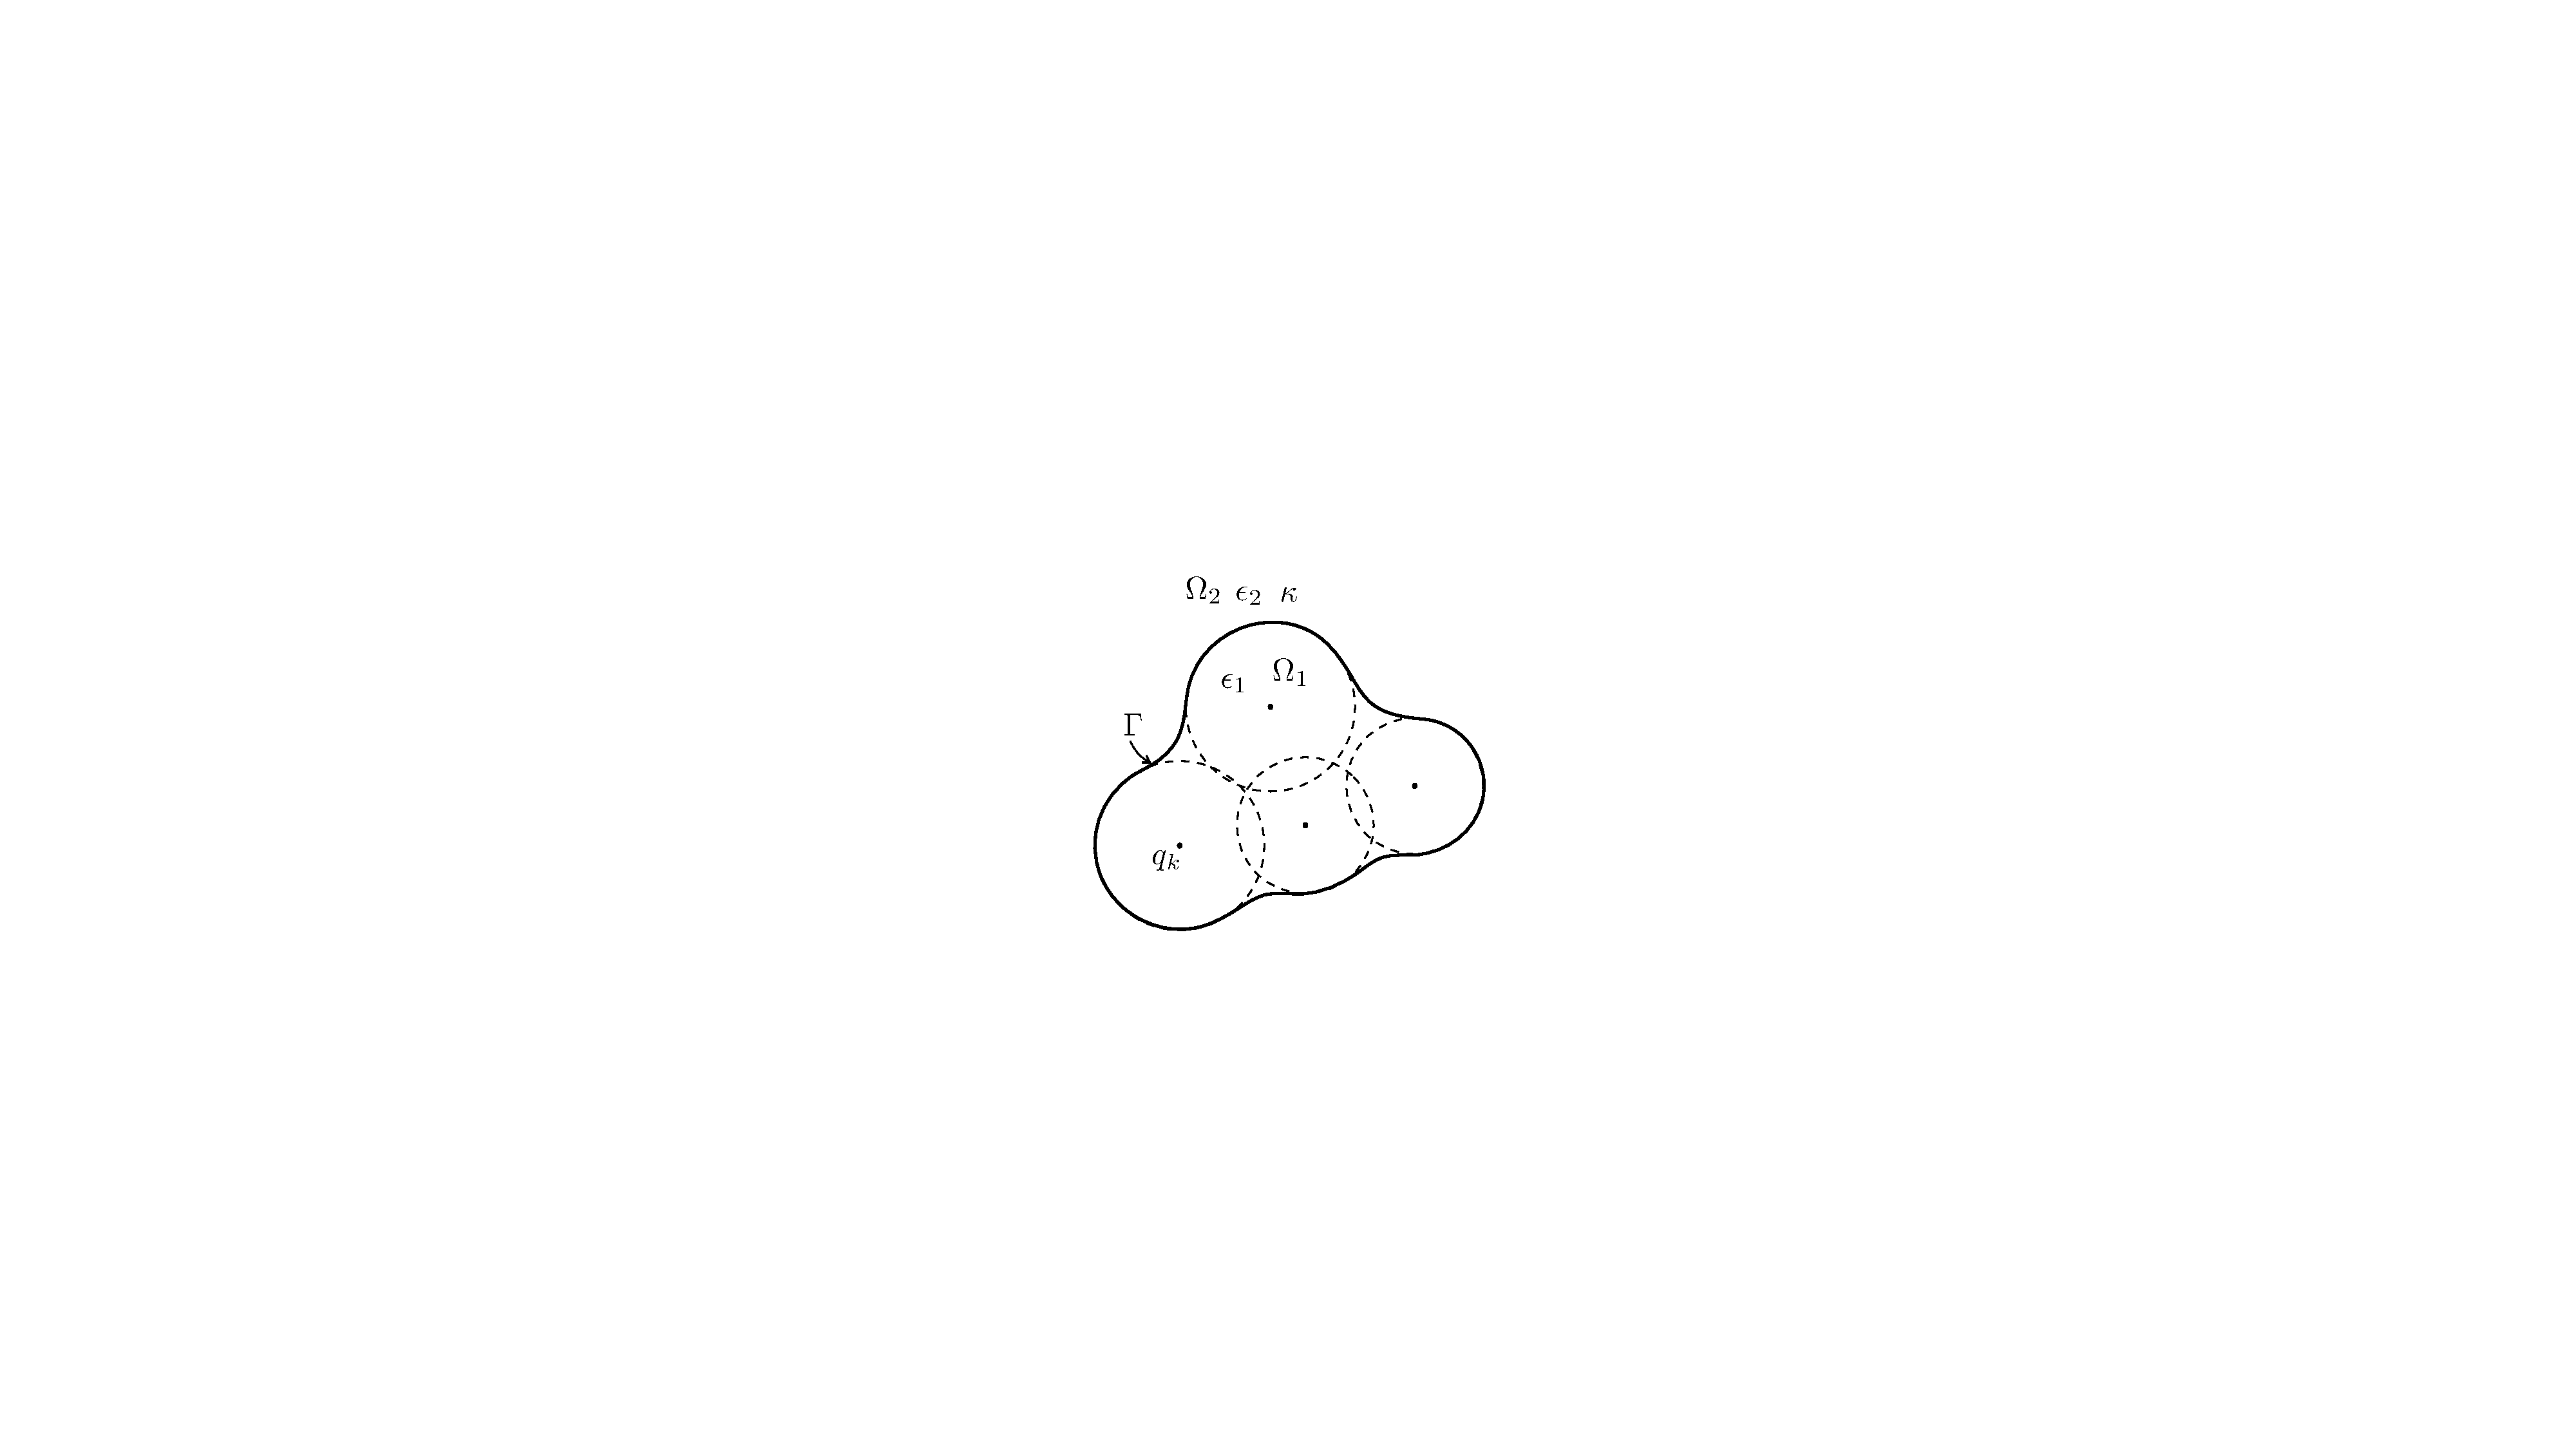
\includegraphics[width=0.3\textwidth]{implicit_molecule.pdf}
\caption{Representation of a molecule in an implicit solvent.}
\label{fig:implicit_molecule}
\end{figure}

The electrostatic potential in $\Omega_1$ can be further decomposed into singular and regular components as $\phi_1 = \phi_c + \phi_r$, where $\phi_c$ is the solution to
%
\begin{align}\label{eq:phic}
\nabla^2\phi_c(\mathbf{x}) &= \tfrac{1}{\epsilon}\sum_{k=1}^{N_q}q_k\delta(\mathbf{x},\mathbf{x}_k) \quad \mathbf{x}\in\Omega_1\cup\Omega_2\nonumber\\
\phi_c(\mathbf{x})&=0 \quad \text{ as } |\mathbf{x}|\to\infty
\end{align}

Physically, $\phi_c$ can be interpreted as the Coulomb-type potential from the point charges, whereas $\phi_r$, also known as reaction potential, is originated by the polarization of the solvent and reorganization of the free ions. 
Usually, $\epsilon_1$ is considered a constant value, yielding an analytical expression for $\phi_c$, however, this is not the general case.

Regularized versions of Equation \eqref{eq:pbe} \cite{LuZhouHolstMcCammon2008,LeeGengZhao2021} are widely used to numerically solve the Poisson-Boltzmann equation with finite element or finite difference methods, and have recently been extended to super-Gaussian permitivitties in the solute.\cite{wang2022regularization} However, here we use the standard formulation in Equation \eqref{eq:pbe}, as it offers more flexibility when dealing with, for example, variable permitivitties, beyond super-Gaussian descriptions.

A common quantity of interest in implicit solvent models is the solvation free energy, which the change in Gibbs free energy as the molecule moves from vacuum into the solvent. Considering the charge distribution $\rho$ consists of point charges, this can be calculated as
%
\begin{equation}\label{eq:dG} 
\Delta G_{solv} = \tfrac{1}{2}\int_{\Omega_1} \rho(\mathbf{x})\phi_{r}(\mathbf{x}) = \tfrac{1}{2}\sum_{k=1}^{N_q} q_k\phi_r(\mathbf{x_k})
\end{equation}

\subsection*{\sffamily \large BEM-BEM coupling}

Several possible boundary integral formulations of Equation \eqref{eq:pbe} exist.~\cite{search2022towards} The simplest form was presented by Yoon ºand Lenhoff in 1991,~\cite{YoonLenhoff1990} known as the \emph{direct} formulation, however, the resulting system is usually ill-conditioned. Here, we use the better-conditioned formulation presented by Lu and co-workers,~\cite{LuETal2006,LuETal2009,debuhr2016dashmm} which reads
%
\begin{align}\label{eq:lu}
    & \tfrac{\phi_2}{2}\left(1+\tfrac{\epsilon_1}{\epsilon_2}\right) - \left(K_Y^\Gamma - \tfrac{\epsilon_1}{\epsilon_2}K_L^\Gamma\right)\phi_2 + \left(V_Y^\Gamma - V_L^\Gamma\right)\lambda_2 = \sum_{k=0}^{N_q}  \frac{q_k}{4\pi\epsilon_2|\mathbf{x}_{\Gamma} - \mathbf{x}_k|}
     \nonumber \\
    &\tfrac{\epsilon_1}{\epsilon_2}\left(W_Y^\Gamma - W_L^\Gamma\right)\phi_2 +  \tfrac{\lambda_2}{2}\left(1+\tfrac{\epsilon_1}{\epsilon_2}\right) + \left(\tfrac{\epsilon_1}{\epsilon_2}K_Y^{\prime\Gamma} - K_L^{\prime\Gamma}\right)\lambda_2 = \sum_{k=0}^{N_q}  \frac{\partial}{\partial\mathbf{n}_\mathbf{x}}\left(\frac{q_k}{4\pi\epsilon_2|\mathbf{x}_{\Gamma} - \mathbf{x}_k|}\right)
\end{align}
%
In Equation \eqref{eq:lu}, $\phi_1 = \phi_1(\mathbf{x}_\Gamma)$ and $\phi_2 = \phi_2(\mathbf{x}_\Gamma)$ are the potentials on $\Gamma$ as we approach from $\Omega_1$ and $\Omega_2$, respectively. For convenience, we call the normal derivative on the interface ({\it ie.} the Neumann trace) $\lambda=\left(\frac{\partial}{\partial \mathbf{n}}  \phi_{\Gamma}  \right)$. $V$, $K$, $K^{\prime}$, and $W$ are the single-layer, double-layer, adjoint double-layer, and hypersingular operators for the Laplace (subscript $L$) and Yukawa (subscript $Y$, also known as modified Helmholtz) kernels. These are defined %in Equation~\eqref{eq:single_double} and 
as
%
\begin{align}\label{eq:all_op}
V_i^\Gamma \varphi (\mathbf{x}) &= \oint_\Gamma g_i(\mathbf{x},\mathbf{x}')\varphi(\mathbf{x}')d\mathbf{x}'\nonumber\\
K_i^\Gamma \varphi (\mathbf{x}) &= \oint_\Gamma \frac{\partial g_i}{\partial\mathbf{n}'}(\mathbf{x},\mathbf{x}')\varphi(\mathbf{x}')d\mathbf{x}',\nonumber\\
K^{\prime\Gamma}_i\varphi (\mathbf{x}) &= \oint_\Gamma \frac{g_i}{\partial\mathbf{n}}(\mathbf{x}_\Gamma,\mathbf{x}')\varphi(\mathbf{x}')d\mathbf{x}'\nonumber\\
W^\Gamma_i\varphi (\mathbf{x}) &= - \oint_\Gamma \frac{\partial^2 g_i}{\partial\mathbf{n}'\partial\mathbf{n}}(\mathbf{x}_\Gamma,\mathbf{x}')\varphi(\mathbf{x}')d\mathbf{x}'
\end{align}
%
where $i \in \{L,Y\}$, $\varphi(\mathbf{x})$ can be any distribution over $\Gamma$, and %Green's functions $g_L, g_Y$ were defined in Equation~\eqref{eq:green_func}.
\begin{align}\label{eq:green_func}
g_L(\mathbf{x},\mathbf{x}')=\frac{1}{4\pi|\mathbf{x}-\mathbf{x}'|} \nonumber \\
g_Y(\mathbf{x},\mathbf{x}')=\frac{e^{-\kappa|\mathbf{x}-\mathbf{x}'|}}{4\pi|\mathbf{x}-\mathbf{x}'|}
\end{align}
are the corresponding free-space Green's functions.

%%Applying Green's second identity to Equation \eqref{eq:pbe} we get 
%%
%%\begin{align} \label{eq:volume_potential}
%%\phi_{1}(\mathbf{x}_{\Omega_1})+ K_{L}^{\Omega_1}\phi_1 -  V_{L}^{\Omega_1} \lambda_2^1 & = \tfrac{1}{\epsilon_1} \sum_{k=0}^{N_q}  \frac{q_k}{4\pi|\mathbf{x}_{\Omega_1} - \mathbf{x}_k|}  \quad \text{on $\Omega_1$,} \nonumber \\
%%\phi_{2}(\mathbf{x}_{\Omega_2}) - K_{Y}^{\Omega_2}\phi_2 + \tfrac{\epsilon_1}{\epsilon_2} V_{Y}^{\Omega_2} \lambda_2& = 0 \quad \text{on $\Omega_2$,}
%%\end{align}
%%
%%where $\mathbf{x}_\Omega$ is evaluated anywhere in the correspoding domain, except $\Gamma$, and $\phi_1 = \phi_1(\mathbf{x}_\Gamma)$ and $\phi_2 = \phi_2(\mathbf{x}_\Gamma)$ are the potentials on $\Gamma$ as we approach from $\Omega_1$ and $\Omega_2$, respectively. For convenience, we call the normal derivative on the interface ({\it ie.} the Neumann trace) $\lambda=\left(\frac{\partial}{\partial \mathbf{n}}  \phi_{\Gamma}  \right)$. $K$ and $V$ are the double- and single-layer potentials for the Laplace (subscript $L$) and Yukawa (subscript $Y$, also known as modified Helmholtz) kernels
%%
%%\begin{align}\label{eq:single_double}
%%V^D \varphi (\mathbf{x}) = \oint_\Gamma g_i(\mathbf{x},\mathbf{x}')\varphi(\mathbf{x}')d\mathbf{x}'\nonumber\\
%%K^D \varphi (\mathbf{x}) = \oint_\Gamma \frac{\partial g_i}{\partial\mathbf{n}'}(\mathbf{x},\mathbf{x}')\varphi(\mathbf{x}')d\mathbf{x}',\nonumber\\
%%\end{align}
%%
%%where $D \in \{\Omega_1, \Omega_2, \Gamma\}$, $i \in \{L,Y\}$, $\varphi(\mathbf{x})$ can be any distribution over $\Gamma$, and 
%%
%%\begin{align}\label{eq:green_func}
%%g_L(\mathbf{x},\mathbf{x}')=\frac{1}{4\pi|\mathbf{x}-\mathbf{x}'|} \nonumber \\
%%g_Y(\mathbf{x},\mathbf{x}')=\frac{e^{-\kappa|\mathbf{x}-\mathbf{x}'|}}{4\pi|\mathbf{x}-\mathbf{x}'|}
%%\end{align}
%%
%%are the free-space Green's function of the Laplace and linearized Poisson-Boltzmann equations, respectively. 
%
%%If we take the limit of Eq. \eqref{eq:volume_potential} as $\mathbf{x}_{\Omega}$ approaches $\Gamma$, we get
%%
%%\begin{align} \label{eq:direct}
%%\tfrac{\phi_1}{2}+ K_{L}^{\Gamma}\phi_1 -  V_{L}^{\Gamma} \lambda_2^1 & = \tfrac{1}{\epsilon_1} \sum_{k=0}^{N_q}  \frac{q_k}{4\pi|\mathbf{x}_{\Gamma} - \mathbf{x}_k|} \nonumber \\
%%\tfrac{\phi_2}{2} - K_{Y}^{\Gamma}\phi_2 +  \tfrac{\epsilon_1}{\epsilon_2} V_{Y}^{\Gamma} \lambda_2 & = 0
%%\end{align}
%%
%%The {\it direct} formulation\cite{YoonLenhoff1990} couples the two expressions of Eq. \eqref{eq:direct} on $\Gamma$, considering the interface conditions. Even though this formulation is poorly conditioned with respect to the mesh size, it can still model large systems when it is preconditioned appropriately.\cite{AltmanBardhanWhiteTidor09,MartinezETal2019,wang2021high} 
%%The formulation presented by Lu\cite{LuETal2006} takes the normal derivative of \eqref{eq:direct} to couple both $\phi$ and $\partial\phi/\partial\mathbf{n}$ as
%%
%%\begin{align}\label{eq:lu}
%%    & \tfrac{\phi_2}{2}\left(1+\tfrac{\epsilon_1}{\epsilon_2}\right) - \left(K_Y^\Gamma - \tfrac{\epsilon_1}{\epsilon_2}K_L^\Gamma\right)\phi_2 + \left(V_Y^\Gamma - V_L^\Gamma\right)\lambda_2 = \sum_{k=0}^{N_q}  \frac{q_k}{4\pi\epsilon_2|\mathbf{x}_{\Gamma} - \mathbf{x}_k|}
%%     \nonumber \\
%%    &\tfrac{\epsilon_1}{\epsilon_2}\left(W_Y^\Gamma - W_L^\Gamma\right)\phi_2 +  \tfrac{\lambda_2}{2}\left(1+\tfrac{\epsilon_1}{\epsilon_2}\right) + \left(\tfrac{\epsilon_1}{\epsilon_2}K_Y^{\prime\Gamma} - K_L^{\prime\Gamma}\right)\lambda_2 = \sum_{k=0}^{N_q}  \frac{\partial}{\partial\mathbf{n}_\mathbf{x}}\left(\frac{q_k}{4\pi\epsilon_2|\mathbf{x}_{\Gamma} - \mathbf{x}_k|}\right)
%%\end{align}
%%
%%The two new integral operators that appear are defined as 
%%
%%\begin{align}
%%\label{eq:adj_hyp}
%%K^{\prime\Gamma}_i\varphi (\mathbf{x}) = \oint_\Gamma \frac{g_i}{\partial\mathbf{n}}(\mathbf{x}_\Gamma,\mathbf{x}')\varphi(\mathbf{x}')d\mathbf{x}'\nonumber\\
%%W^\Gamma_i\varphi (\mathbf{x}) = - \oint_\Gamma \frac{\partial^2 g_i}{\partial\mathbf{n}'\partial\mathbf{n}}(\mathbf{x}_\Gamma,\mathbf{x}')\varphi(\mathbf{x}')d\mathbf{x}'
%%\end{align}
%%where $i \in \{L,Y\}$, 
%%and are called the {\it  adjoint double layer} and {\it hypersingular} operators, respectively. Note that the potential in Eq. \eqref{eq:lu} is evaluated on the exterior. 
%
%In weak form, Eq. \eqref{eq:lu} becomes
%%
%\begin{align}\label{eq:lu_disc}
%&\left< \left(1+\tfrac{\epsilon_1}{\epsilon_2}\right) \tfrac{\phi_{2}}{2} - \left(K_Y^\Gamma - \tfrac{\epsilon_1}{\epsilon_2}K_L^\Gamma\right)\phi_{2}, v \right>_{\Gamma} + \left< \left(V_Y^\Gamma - V_L^\Gamma\right) \lambda_2, v \right>_\Gamma = \left< \sum_{k=0}^{N_q}  f_k, v \right>_{\Gamma} \nonumber \\
%&\left< \tfrac{\epsilon_1}{\epsilon_2}\left(W_Y^\Gamma - W_L^\Gamma\right)\phi_{2}, \zeta \right>_\Gamma + \left<  \left(1+\tfrac{\epsilon_1}{\epsilon_2}\right) \tfrac{\lambda_2}{2} + \left(\tfrac{\epsilon_1}{\epsilon_2}K_Y^{\prime\Gamma} - K_L^{\prime\Gamma}\right)\lambda_2, \zeta\right>_\Gamma = \left< \sum_{k=0}^{N_q}  \frac{\partial}{\partial\mathbf{n}_\mathbf{x}} f_k, \zeta \right>_{\Gamma}
%\end{align}
%%
%where $v, \zeta$ are test functions, $\left<\varphi,v\right>_\Gamma = \int_\Gamma \varphi(\mathbf{x})v(\mathbf{x})d\mathbf{x}$ %and $\left(\varphi,v\right)_\Omega = \int_\Omega \varphi(\mathbf{x})v(\mathbf{x})d\mathbf{x}$ are 
%is the inner products on the surface% and domain, respectively
%and $f_k := \frac{q_k}{4\pi\epsilon_2|\mathbf{x}_{\Gamma} - \mathbf{x}_k|}$.
%
%We introduce below the matrix formulation. Let $\vec{\phi}_2 := [\phi_2^1, \dots, \phi_2^k]^T$ be the vector of canonical basis
%functions of $W_{h}^{k}$ and  $\vec{\lambda}_2 := [\lambda_2^1, \dots, \lambda_2^l]^T$ - the vector of canonical basis
%functions of $\Lambda_{h}^{l}$. We define the following matrices associated with the corresponding bilinear forms
%\begin{align*}
%\widetilde{K}_{\alpha \beta} = \left<\left(K_Y^\Gamma - \tfrac{\epsilon_1}{\epsilon_2}K_L^\Gamma\right) \phi^{\alpha}_2, \ \lambda^{\beta}_2 \right>_{\Gamma}
% &,&
%\widetilde{V}_{\alpha \beta} = \left<\left(V_Y^\Gamma - V_L^\Gamma\right) \lambda^{\alpha}_2, \ \lambda^{\beta}_2 \right>_{\Gamma}, \\
%\widetilde{W}_{\alpha \beta} = \left<\left(W_Y^\Gamma - W_L^\Gamma\right) \phi^{\alpha}_2, \ \phi^{\beta}_2 \right>_{\Gamma}
% &,&
%\widetilde{K'}_{\alpha \beta} = \left<\left(\tfrac{\epsilon_1}{\epsilon_2}K_Y^{\prime\Gamma} - K_L^{\prime\Gamma}\right) \lambda^{\alpha}_2, \ \phi^{\beta}_2 \right>_{\Gamma},
%\end{align*}
%and vectors associated with the corresponding linear forms
%\begin{align*}
%\vec{f}_{\beta} = \left< \sum_{k=0}^{N_q}  \frac{q_k}{4\pi\epsilon_2|\mathbf{x}_{\Gamma} - \mathbf{x}_k|},   \phi^{\beta}_1  \right>_{\Gamma} &,& \vec{\partial f}_{\beta} = \left< \sum_{k=0}^{N_q}  \frac{\partial}{\partial\mathbf{n}_\mathbf{x}}\left(\frac{q_k}{4\pi\epsilon_2|\mathbf{x}_{\Gamma} - \mathbf{x}_k|}\right),   \phi^{\beta}_1  \right>_{\Gamma}.
%\end{align*}
%
%Using the above definition the discrete problem~\eqref{eq:fem_bem_disctrete} can be written in the following matrix form
%\begin{align*}
%\begin{bmatrix}
% \tfrac12 \left(1+\tfrac{\epsilon_1}{\epsilon_2}\right) I - \widetilde{K}  & \widetilde{V}  \\  
% \tfrac{\epsilon_1}{\epsilon_2} \widetilde{W} & \tfrac12 \left(1+\tfrac{\epsilon_1}{\epsilon_2}\right) I + \widetilde{K'}
%\end{bmatrix}
%\begin{bmatrix}
%\vec{\phi}_2 \\
%\vec{\lambda}_2 
%\end{bmatrix}
%= 
%\begin{bmatrix}
%\vec{f} \\  
%\vec{\partial f}
%\end{bmatrix}.
%\end{align*}
%%
%

Having computed the electrostatic potential with Eq. \eqref{eq:lu}, we obtain the reaction potential ($\phi_r$) in Eq. \eqref{eq:dG} by subtracting out the Coulombic component out of $\phi_1$. This gives\cite{CooperBardhanBarba2014}
%
\begin{align} \label{eq:phi_reac}
\phi_{r}(\mathbf{r}) = - K_{L}^{\mathbf{r}} \phi_1 + V_{L}^{\mathbf{r}}  \lambda_1  ,
\end{align}
%
where $\mathbf{r}\in\Omega_1$.
This is valid as long as $\epsilon_1$ is a constant. We use Eq.~\eqref{eq:phi_reac} for both BEM-BEM and FEM-BEM coupling simulations with constant $\epsilon_1$.



\subsection*{\sffamily \large Novel numerical solution of the Poisson-Boltzmann equation}

%\subsection*{\sffamily \normalsize FEM-BEM coupling}

The boundary element method (BEM) is a standard tool for the numerical solution of the Poisson-Boltzmann equation in molecular electrostatics.~\cite{ZauharMorgan1985, Shaw1985} This was implemented in numerous codes, such as AFMPB,~\cite{LuETal2006} TABI,~\cite{GengKrasny2013} PyGBe,~\cite{CooperBardhanBarba2014,cooper2016pygbe} and more recently, with Bempp-cl.~\cite{search2022towards}. Its popularity comes because it reduces the dimension of the problem by using the boundary integral formulation. Unfortunately, this advantage comes at a cost: it requires a fundamental solution to be applied. There are many linear problems for which fundamental solutions are not known, for example, this is the case for the Poisson-Boltzmann equation with a heterogenous permittivity inside the molecule
%
   \begin{align} \label{eq:pbe_vp}
\nabla \cdot \left(\epsilon_1(\mathbf{x}) \nabla \phi_1(\mathbf{x})\right) &= \sum_{k=1}^{N_q} q_k\delta(\mathbf{x},\mathbf{x}_k) \quad  \mathbf{x} \in \Omega_1\nonumber\\
\left(\nabla^2 - \kappa^2\right)\phi_2(\mathbf{x})  &= 0 \quad\mathbf{x}\in\Omega_2\nonumber\\
\phi_1(\mathbf{x})  = \phi_2(\mathbf{x}),  &\quad \epsilon_1(\mathbf{x})\frac{\partial\phi_1}{\partial\mathbf{n}}(\mathbf{x})  = \epsilon_2(\mathbf{x})\frac{\partial\phi_2}{\partial\mathbf{n}}(\mathbf{x})  \quad \mathbf{x}\in \Gamma. 
\end{align}
%
A finite element method (FEM) is more suitable for such case.

The coupling of finite element (FEM) and boundary element (BEM) methods is a widely used approach to solve multi-physical problems on unbounded domains [citation?], as it takes advantage of both methods. On one hand, the BEM satifies the infinite boundary conditions exactly when they decay to zero, and only approximates boundary conditions on surfaces, hence, it is commonly used for problems involving infinite or semi-infinite domains. On the other hand, the FEM is known for its robustness and universal applicability, even for problems of inhomogeneous or non-linear nature.
Here, we used the Johnson-N\'ed\'elec formulation,\cite{johnson1980coupling} which is the simplest form of FEM-BEM coupling, and we detail it next.

   We start with the variational formulation of the internal problem. Applying integration by parts for first equation of~\eqref{eq:pbe_vp} for every $v \in H_0^1(\Omega_1)$, we have
% 
\begin{equation}
\label{eq:fem}
 \left( \epsilon_1 \nabla \phi_1, \nabla v \right)_{\Omega_1}  -  \left<  \epsilon_1\partial_n \phi_1, v \right>_\Gamma =  \left( \sum_{k=1}^{N_q} q_k\delta(\mathbf{x},\mathbf{x}_k),  v\right)_{\Omega_1},
\end{equation}
%
where $v$ is a test function, and $\left<\varphi,v\right>_\Gamma = \int_\Gamma \varphi(\mathbf{x})v(\mathbf{x})d\mathbf{x}$ and $\left(\varphi,v\right)_{\Omega_1} = \int_{\Omega_1} \varphi(\mathbf{x})v(\mathbf{x})d\mathbf{x}$ are the inner products on the surface and domain, respectively.
For the external problem with BEM, we define the Dirichlet trace~\cite{MR2361676} 
\begin{align*}
% \label{eq:trace_map}
\gamma:  H^1(\Omega_2) &\rightarrow H^{\frac{1}{2}}(\Gamma) & \gamma f(x) & := \lim_{\Omega_2 \ni y \rightarrow x \in \Gamma}  f(y),
\end{align*}
and we use the direct formulation from the second equation of Eq.~\eqref{eq:pbe} to obtain
\begin{align*}
\tfrac{\phi_1}{2} - K_{Y}^{\Gamma}\gamma \phi_1 + \tfrac{\epsilon_1}{\epsilon_2}V_{Y}^{\Gamma}  \lambda_1 & = 0.
\end{align*}
$V$ and $K$ are the single-layer and double-layer operators for the Laplace (subscript $L$) and Yukawa (subscript $Y$, also known as modified Helmholtz) kernels. These are defined in Equations~\eqref{eq:all_op} and~\eqref{eq:green_func}.
%as
%
%\begin{align}\label{eq:single_double}
%V_i^\Gamma \varphi (\mathbf{x}) &= \oint_\Gamma g_i(\mathbf{x},\mathbf{x}')\varphi(\mathbf{x}')d\mathbf{x}'\nonumber\\
%K_i^\Gamma \varphi (\mathbf{x}) &= \oint_\Gamma \frac{\partial g_i}{\partial\mathbf{n}'}(\mathbf{x},\mathbf{x}')\varphi(\mathbf{x}')d\mathbf{x}',\nonumber\\
%K^{\prime\Gamma}_i\varphi (\mathbf{x}) &= \oint_\Gamma \frac{g_i}{\partial\mathbf{n}}(\mathbf{x}_\Gamma,\mathbf{x}')\varphi(\mathbf{x}')d\mathbf{x}'\nonumber\\
%W^\Gamma_i\varphi (\mathbf{x}) &= - \oint_\Gamma \frac{\partial^2 g_i}{\partial\mathbf{n}'\partial\mathbf{n}}(\mathbf{x}_\Gamma,\mathbf{x}')\varphi(\mathbf{x}')d\mathbf{x}'
%\end{align}
%
%where $i \in \{L,Y\}$, $\varphi(\mathbf{x})$ can be any distribution over $\Gamma$, and
%
%\begin{align}\label{eq:green_func}
%g_L(\mathbf{x},\mathbf{x}')=\frac{1}{4\pi|\mathbf{x}-\mathbf{x}'|} \nonumber \\
%g_Y(\mathbf{x},\mathbf{x}')=\frac{e^{-\kappa|\mathbf{x}-\mathbf{x}'|}}{4\pi|\mathbf{x}-\mathbf{x}'|}
%\end{align}
%
%are the corresponding free-space Green's functions.

Then, the coupling problem can be written as
%
\begin{center}
  \textit{Find $ \phi_1 \in H^1(\Omega_1)$ and $\lambda_2 \in H^{-\frac{1}{2}}(\Gamma)$ such that for all $v \in H^1(\Omega_1)$ and $\zeta \in H^{-\frac{1}{2}}(\Gamma)$}
\begin{equation} 
\label{eq:standard_fem_bem}
 \left\{
 \begin{array}{rcl}
 \left(  \epsilon_1 \nabla \phi_1, \nabla v \right)_{\Omega_1}  - \left< \epsilon_1 \lambda_2, v \right>_\Gamma &=&   \left(  \sum_{k=1}^{N_q} q_k\delta(\mathbf{x},\mathbf{x}_k),  v \right)_{\Omega_1} \\[3mm] 
  \left< \left(\tfrac{1}{2} I - K_{Y}^{\Gamma}\right) \gamma \phi_1, \zeta \right>_\Gamma + \tfrac{\epsilon_1}{\epsilon_2} \left< V_{Y}^{\Gamma} \lambda_2, \zeta \right>_\Gamma &=&0.
  \end{array}
  \right.
\end{equation}
\end{center}


%\begin{align}\label{eq:standard_fem_bem}
% \int_{\Omega_1} \epsilon_1 \nabla \phi_1 : \nabla v ~d\mathbf{x}  - \oint_\Gamma \epsilon_1\partial_n \phi_1 v ds &=   \int_{\Omega_1}  \sum_{k=1}^{N_q} q_k\delta(\mathbf{x},\mathbf{x}_k)  v ~d\mathbf{x} \\
% \oint_\Gamma \tfrac{\phi_1}{2} - K_{Y}^{\Gamma}(\phi_1) + \tfrac{\epsilon_1}{\epsilon_2}V_{Y}^{\Gamma} \left( \lambda_2^1 \right) & = 0
%\end{align}

This can also be written in matrix form. Let $\vec{\phi}_1 := [\phi_1^1, \dots, \phi_1^j]^T$ be the vector of canonical basis
functions of the finite element space $V_{h}^{j}$, %$\vec{\phi}_2 := [\phi_2^1, \dots, \phi_2^k]^T$ - the vector of canonical basis functions of $W_{h}^{k}$,  
$\vec{\lambda}_2 := [\lambda_2^1, \dots, \lambda_2^l]^T$ --- the vector of canonical basis
functions of $\Lambda_{h}^{l}$. % and $\vec{\widetilde{\phi}} := [\widetilde{\phi}^1, \dots, \widetilde{\phi}^m]^T$ be the vector of canonical basis functions of  $M_{h}^{m}$
% $T:\Omega_1 \rightarrow \Gamma$ and $E:\Gamma \rightarrow \Omega_1$ trace and extendable operators respectively.
We define the following matrices associated with the corresponding bilinear forms
\begin{align*}
A_{\alpha \beta} = \left(\nabla \phi_1^{\alpha}, \nabla \phi_1^{\beta} \right)_{\Omega_1}  
&,&
M_{\alpha \beta} = \left< \widetilde{\phi}^{\alpha}, \ \lambda^{\beta}_2 \right>_{\Gamma}, \\
K_{\alpha \beta} = \left<K_{Y}^{\Gamma} \gamma \phi^{\alpha}_1, \ \lambda^{\beta}_2 \right>_{\Gamma}
 &,&
V_{\alpha \beta} = \left<V_{Y}^{\Gamma} \lambda^{\alpha}_2, \ \lambda^{\beta}_2 \right>_{\Gamma}, 
\end{align*}
and vector associated with the corresponding linear form
\begin{equation*}
\vec{f}_{\beta} := \left(  \sum_{k=1}^{N_q} q_k\delta(\mathbf{x},\mathbf{x}_k),  \phi_1^{\beta} \right)_{\Omega_1}.
\end{equation*}
Using the above definition the discrete problem in Eq.~\eqref{eq:standard_fem_bem} can be written in the following matrix form
\begin{align*}
\begin{bmatrix}
\epsilon_1 A &  - \epsilon_1 M^T \\  
\left(\tfrac12 I + K \right) \gamma &  \tfrac{\epsilon_1}{\epsilon_2} V 
\end{bmatrix}
\begin{bmatrix}
\vec{\phi}_1 \\  
\vec{\lambda}_2
\end{bmatrix}
= 
\begin{bmatrix}
\vec{f} \\  
0
\end{bmatrix}.
\end{align*}

